% \documentclass{article}
% Tipo di documento. L'uso di twoside implica che i capitoli inizino sempre con la prima pagina a sinistra, eventualmente lasciando una pagina vuota nel capitolo precedente. Se questa cosa è fastidiosa, è possibile rimuoverlo. 
% \documentclass[a4paper, twoside,openright]{report}
\documentclass[a4paper,openright]{report}

\usepackage{graphicx} % Required for inserting images

\usepackage[utf8]{inputenc}

\usepackage{hyperref}

\usepackage{graphicx}
\setkeys{Gin}{width=0.6\textwidth}

\usepackage{wrapfig}

\usepackage{enumitem}
\usepackage{paracol}
\usepackage{multicol}

\usepackage{geometry}

\usepackage{color}

\usepackage{listings}

\usepackage{amsmath}
\usepackage{mathtools}
\usepackage{bm}

\usepackage{soul}
\usepackage{booktabs}

\usepackage{rotating}
\usepackage{adjustbox}

% Uso dei colori
\usepackage[dvipsnames]{xcolor}

\usepackage{tikz}
\usetikzlibrary{automata, arrows}
\usetikzlibrary{positioning}
\usetikzlibrary{shapes.geometric}

\geometry{margin=0.6in}

\setlist[description]{itemsep=0em,topsep=0.5em,parsep=0em}
\setlist[itemize]{itemsep=0em}

\hypersetup{
    colorlinks=true,
    linkcolor=black,
    filecolor=mauve,
    urlcolor=blue,
}

\definecolor{gray}{gray}{0.3}
\definecolor{OliveGreen}{rgb}{0,0.6,0}
\definecolor{mauve}{rgb}{0.58,0,0.82}
\definecolor{darkred}{rgb}{0.3,0,0}
\definecolor{darkgreen}{rgb}{0,0.3,0}


\newenvironment{notes}{
\par
\color{gray}
\small}

\newcommand{\note}[1]{\begin{notes}{#1}\end{notes}}
\newcommand{\lst}[1]{\lstinline{#1}}
\newcommand{\nl}[0]{\parskip = \baselineskip}

\newcommand{\labelitemize}[2]{
\newlength{\currentparindent}
\setlength{\currentparindent}{\parindent}
\setlength{\parindent}{0pt}

\begin{minipage}{0em} % Adjust the width as needed
    \makebox[0em][c]{\rotatebox{90}{\small #1}}
\end{minipage}
\begin{minipage}{\dimexpr\textwidth-1cm\relax}
    #2
\end{minipage}
\setlength{\parindent}{\currentparindent}
\undef{\currentparindent}
}

\lstset{frame=false,
 showstringspaces=false,
 breaklines=true;
 columns=flexible,
 basicstyle={\small\ttfamily},
 keywordstyle=\color{blue},
 commentstyle=\color{dkgreen},
 stringstyle=\color{mauve}
 tabsize=3
}

\title{Advanced Software Engineering - Appunti}
\author{Francesco Lorenzoni}
\date{September 2023}

\begin{document}

\maketitle
\tableofcontents

\chapter{Introduction}

Prof. Cisternino dropped a lot of measures in terms of Watts, Dollars, Gigabits and so on.

He mentioned with emphasis the problem of energy consumption.
To give an idea, a single rack of a datacenter designed $\sim10$ years ago, absorbs \ul{up to $15kW$}.
The datacenter in \textit{San Piero a Grado} is made up of 60 racks. It is not meant to provide the maximum energy possible for all racks simultaneously, but it still helps to get an idea of how things work in similar contexts.

\section{Course map}
\begin{enumerate}
   \item Elements
   \begin{enumerate}
      \item Datacenters
      \begin{enumerate}
         \item Power
         \item Cooling
      \end{enumerate}
      \item Cabling
      \item Networking
      \item Storage
      \item Compute
      \item Virtualization
      \begin{enumerate}
         \item Hypervisor
         \item Containers
      \end{enumerate}
   \end{enumerate}
   \item Cloud
   \begin{enumerate}
      \item Reference architecture
      \item Resilience
      \item Security
      \item Legal aspects
      \begin{enumerate}
         \item GDPR
         \item Security frameworks
      \end{enumerate}
      \item Procurement aspects
      \item Operations
      \note{i.e. Keep the system up and running while upgrading the system}
   \end{enumerate}
\end{enumerate}
\chapter{Distributed Hash Tables}
\begin{figure}[htbp]
   \centering
   \includegraphics{images/DHT_motivations.png}
   \caption{DHT Motivations}
   \label{fig:DHT_motivations}
\end{figure}

The key idea is to split the hash tables into several parts and distribute them to several servers, and to use hash of resources (or of the URLs of resources) as a key to map them to a
dynamically changing set of web caches, but with \ul{each key mapped to single server}; so that
each machine (user) can locally compute which web cache should contain the
required resource, refenced by an URL.\\
This technique is extended to DHT for P2P systems.

However, \ul{\textbf{rehashing} is a problem in dynamic scenarios} if the hashing scheme depends directly on the number of servers:
$99\%$ of keys have to be remapped, resulting in a lot of messages exchange.
\begin{figure}[htbp]
   \centering
   \includegraphics{images/rehashing_problem.png}
   \caption{Rehashing problem}
   \label{fig:rehashing_problem}
\end{figure}

\textbf{Consistent hashing} is a set of hash techniques which guarantees that adding more nodes/remove nodes implies \ul{moving only a minority of data items}.
each node manages ---instead of a set of sparse keys--- an interval of consecutive hash keys, and intervals are joined/splitted when nodes join/leave the network and keys redistributed between adjacent peers.


\section{Building DHT}
\begin{paracol}{2}
   % \colfill
   \begin{itemize}
      \item Use a logical name space, called \textit{identifier space} consisting of identifiers
      $\{0,1,2,...,N-1\}$
      \item define identifier space as a \textit{logical ring} modulo $N$
      \item every node picks a random identifier
      through Hash function $H$.
      \item the function \texttt{succ(x)} returns the node with an identifier $\geq x$.
      \item every item $v$ to be stored gets assigned to \texttt{succ(H(v))}
   \end{itemize}
   \begin{figure}[htbp]
      \centering
      \includegraphics{images/DHT_build2.png}
      % \caption{}
      \label{fig:DHT_build2}
   \end{figure}

   % \colfill
   \switchcolumn
   
   % \begin{adjustbox}{valign=\fill}
   \begin{figure}[htbp]
      \centering
      \includegraphics{images/DHT_build1.png}
      \caption{Identifier space}
      In this figure, the node identifiers are 16 and the green circles indicate which are the online nodes.
      \label{fig:DHT_build1}
   \end{figure}
   % \end{adjustbox}
   
\end{paracol}

\subsection{Peers joining and leaving}
When a new node is \textbf{added}, we map the keys between the new node and the previous node in the hash ring to point to the new node;\\
those the keys will no longer be associated with their old nodes.

When a node is \textbf{removed} from the hash ring, only the keys associated with that node are rehashed and remapped rather than remapping all the keys.

In case a node suddenly disconnects from the network, all data stored on it are lost if they are not stored on other nodes;
to avoid such a problem:
\begin{itemize}
   \item introduce some redundancy (data replication)
   \item information loss: periodical information refresh
\end{itemize}

\begin{figure}[htbp]
   \centering
   \includegraphics{images/p2p_peerleaves.png}
   \caption{Peer 11 leaves the Network}
   \label{fig:p2p_peerleaves}
   In case a peer leaves, its keys can easily be remapped to its successor
\end{figure}

When the hash table is \textbf{resized}, on the average,only $\frac{k}{n}$ keys need to be remapped on average, where $k$ is the number of keys and $n$ is the number of servers.
\newpage
\section{Data Lookup}
\begin{figure}[htbp]
   \centering
   \includegraphics{images/dht_exponentialsearch.png}
   \caption{Exponential Search for DHT}
   The data lookup can be implemented by using exponential search, rather than performing a walk by asking each peer for its successor
   \label{fig:dht_exponentialsearch}
\end{figure}

Data Lookup can be sped up even more, by computing the hash $h(x)$ of the searched object, and propagating the query to farthest node\footnote{Which is found using exponential search} which has an identifier smaller than $h(x)$, which then recursively applies the same algorithm, until the object is found.
\begin{figure}[htbp]
   \centering
   \includegraphics[width=0.3\columnwidth]{images/dht_chordsearch01.png}
   \includegraphics[width=0.3\columnwidth]{images/dht_chordsearch02.png}\\
   \includegraphics[width=0.3\columnwidth]{images/dht_chordsearch03.png}
   \includegraphics[width=0.3\columnwidth]{images/dht_chordsearch04.png}
   \caption{Lookup performed in the \texttt{\textbf{CHORD}} DHT}
   \label{fig:dht_chordsearch}
\end{figure}

\subsection{Addressing data}
Data was usually addressed by \textbf{location}, a \texttt{http://} link to locate resources;
Such link is an identifier that points to a particular location on the web.\\
This approach forces us all to \ul{pretend that the data are in only one location}.

IPFS instead uses \textbf{content addressing}, which exploits the cryptographic hash of the content to identify it.

\subsection{API, Lookup and Various Properties}
To avoid having a node managing a bigger portion of the identifier space, a uniform hash function may be used.\\
Most DHT provide a simple inferface \texttt{PUT,GET,Value}, usually \textit{without} the possibility to move keys.

\begin{figure}[htbp]
   \centering
   \includegraphics{images/DHT_lookupcomplexity.png}
   \caption{Lookup time complexity comparison}
   \label{fig:DHT_lookupcomplexity}
\end{figure}

\labelitemize{\textit{DHT}}{
   \begin{itemize}
      \item Routing is based on key (unique identifier)
      \item Key are uniformly distributed to the DHT nodes
      \begin{enumerate}
         \item Bottleneck avoidance
         \item Incremental insertion of the keys
         \item Fault tolerance
      \end{enumerate}
      \item Auto organizing system
      \item Simplex and efficient organization
      \item The terms “Structured Peer-to-Peer“ and “DHT“ are often used as
      synonyms
   \end{itemize}
}
\chapter{ZigBee}

ZigBee is widely used in various fields from home automation to Mars exploration; it is considered the ``cousin'' of Bluetooth: they are standardized by the same company and can coexist.

\begin{paracol}{2}

   \colfill
   Aside from the application layer, ZigBee defines also a \textit{Network Layer} which perfectly matches and maps to the underlying MAC and Physical Layers, standardized by \texttt{IEEE 802.15.4};
   ZigBee is built on top of such IEEE standard.
   \colfill

   \switchcolumn
   
   \begin{figure}[htbp]
      \centering
      \includegraphics{images/zigbee_layers.png}
      \caption{ZigBee layers}
      \label{fig:zigbee_layers}
   \end{figure}
\end{paracol}

\labelitemize{\textit{Key Features}}{
   \begin{itemize}
      \item Specification of the physical and MAC layers for low-rate Wireless Personal Area Networks (PAN)
      \item Infrastructure-less
      \item Short range\footnote{250m outdoors in ideal conditions}
      \item Support for star and peer-to-peer topologies
      \item Can coexist with IEEE 802.11 and IEEE 802.15.1 (Bluetooth)
      \item Works on licence-free frequency bands
   \end{itemize}
}

\section{Architecture}

\begin{paracol}{2}
   
   
   APS provides \textit{transport} services to the ZDO and the Objects in the Application Framework (APOs). It is some kind of Transport layer, similar to TCP but not the same.
   
   APOs are the business logic of the business device, implemented by the user, and in a single device there may be instantiated up to APOs.
   We may say that for each APO provides a ``functionality''.
   
   The ZDO is an applicative object that defines and maintaines the device behaviour in a ZigBee network.
   \note{An example of this behaviour, is replying to a device discovery message. Such reply is handled by the ZDO}
   The ZDO is provided by the third parties which are giving you the ZigBee stack.
   Manufacturers which produce devices compliant with ZigBee, sell them with a ZigBee stack already implemented, allowing for the buyer ---e.g. a company which develops ZigBee solutions--- to simply implement the ``functionalities'' (i.e. APOs) they want.
   \switchcolumn

   \begin{figure}[htbp]
      \centering
      \includegraphics{images/zigbee_architecture.png}
      \caption{Zigbee architecture layers}
      \label{fig:zigbee_architecture}
   \end{figure}
\end{paracol}

\section{Primitives}
\begin{figure}[htbp]
   \centering
   \includegraphics{images/zigbee_primitives.png}\\
   \includegraphics{images/zigbee_primitives2.png}
   \caption{Mapping between zigbee primitives}
   \label{fig:zigbee_primitives}
\end{figure}

\labelitemize{Primitives}{
   \begin{enumerate}
      \item \texttt{Request}\\
      It is invoked by the upper layer to request for a specific service
      \item \texttt{Indication}\\
      Is a sort of \textit{``upcall''}, generated by the lower layer and is directed to the upper layer to notify the occurrence of an event related to a specific service
      \item \texttt{Response}\\
      It is invoked by the upper layer to complete a procedure previously initiated by an indication primitive
      \item \texttt{Confirm}\\
      It is generated by the lower layer and is directed to the upper layer to convey the results of one or more associated previous service requests.
   \end{enumerate}
}

\section{Network Layer}

The ZigBee network layer provides services for:
\begin{enumerate}
   \item Data transmission (both unicast and multicast)
   \item Network initialization
   \item Devices addressing
   \item Routes management \& routing
   \item Management of joins/leaves of devices
\end{enumerate}

In a ZigBee network there are three kinds of devices:
\begin{enumerate}
   \item \textbf{The Network coordinator}
      
   A FFD\footnote{Full functional Device} that creates and manages the entire network
   \item \textbf{Routers}
      
   A FFD with routing capabilities
   \item \textbf{End-devices}
   
   Correspond to a RFD\footnote{Reduced functional device} or to a FFD acting as simple devices
\end{enumerate}

\begin{figure}[htbp]
   \centering
   \includegraphics{images/zigbee_networktopologies.png}
   \caption{ZigBee Network topologies outline}
   \label{fig:zigbee_networktopologies}
   The superframe mentioned above, is a feature used to obtain energy efficiency in ZigBee networks, but we will discuss it later on.
\end{figure}

\subsection{Network formation and joining}
Before communicating on a network, a ZigBee device must either:
\begin{itemize}
   \item Form a new network $\longrightarrow$ \textit{ZigBee Coordinator}
   \item Join an existing network $\longrightarrow$ \textit{ZigBee router} or \textit{end-device}
\end{itemize}
\note{The role of the device is chosen at compile-time}

\subsubsection{Formation}
\begin{paracol}{2}
   \colfill
   \textbf{Network Formation} is performed by a coordinator, which uses the MAC layer services to (\texttt{SCAN.request}) look for a channel that does not conflict with other existing networks, and then selects a PAN identifier which is not already in use by other PANs.
   \colfill
   \switchcolumn
   \begin{figure}[htbp]
      \centering
      \includegraphics{images/zigbee_netformation.png}
      \caption{Network formation messages}
      \label{fig:zigbee_netformation}
   \end{figure}
\end{paracol}

\subsubsection{Joining}
\begin{paracol}{2}
   \colfill
   Joining may happen in two ways, the first is to \ul{join through \textbf{association}}: 
   initiated by a device wishing to join an existing network.
   
   Alternatively a device may \ul{perform a 
\textbf{Direct join}}:
   requested by a router or by the coordinator to request a device to join its PAN.
   \colfill
   \switchcolumn
   \begin{figure}[htbp]
      \centering
      \includegraphics{images/zigbee_netjoining.png}
      \caption{Network joining messages}
      \label{fig:zigbee_netjoining}
   \end{figure}
\end{paracol}

\section{Application Layer}

Up to 240 APOs, each corresponding to an application \textbf{Endpoint}, with the Endpoint 0 reserved for the ZDO\footnote{We could say that the ZDO is an ``application object'', which would be true, but tailored to specific needs}.
\ul{Each APO in the network is uniquely identified by its endpoint address and the network address} of the hosting device.

\subsection{APS - Application Support Sublayer}
The APS frame uses the concepts of \textbf{endpoints}, \textbf{cluster
ID}s, \textbf{profile ID}s and \textbf{device ID}s.\\
It provides:
\begin{itemize}
   \item Data service (a light transport layer)
   \begin{itemize}
      \item Filtering out packets (non registered endpoints, profiles that do
      not match)
      \item Generating end-to-end acknowledgments
   \end{itemize}
   \item Management:
   \begin{itemize}
      \item Local binding table
      \item Local groups table
      \item Local address map
   \end{itemize}
\end{itemize}

\subsubsection{Concepts and related IDs}

\begin{paracol}{2}
   A \textbf{cluster} may be, in the simplest case, a \textit{message}. But this is not necessarily the case.\\
   Informally, a cluster provides access to a service (a functionality) of an application object;
   \ul{Defines both \textit{commands}}, which cause actions on a device, \ul{and \textit{attributes}}, showing the state of a device in a given cluster.\\
   \note{\ul{Every cluster has a 16 bit identifier}, which according to prof. Chessa is \textbf{not} sufficient.}
   
   Note that clusters are not related to the physical world interaction, because they must allow reuse.\\
   Each cluster finds a possibly different meaning in each \textbf{application profile}. There is a mapping which defines such meanings mappings.
   \note{Using this schema, 16 bits become sufficient.}
   
   An \textbf{application profile} is the specification of the
   behaviour of a class of applications possibly operating
   on several ZigBee devices.
   Each profile is paired with a 16 bit identifier.
   \note{Every message sent (or received) is tagged with a profile ID.
   Different application profiles may co-exist in a single
   ZigBee network.}
   \switchcolumn

   \begin{figure}[htbp]
      \centering
      \includegraphics{images/zigbee_generalclusters.png}\\
      \includegraphics{images/zigbee_appprofiles.png}
      \caption{ZigBee General Domain clusters and common Profile IDs}
      \label{fig:zigbee_generalclusters}
   \end{figure}
\end{paracol}

\begin{paracol}{2}
   ZigBee \textbf{Device ID}s range from \texttt{0x0000} to \texttt{0xFFFF}, and have two purposes:
   \begin{enumerate}
      \item To allow human-readable displays (e.g., an icon related to a device)
      \item Allows ZigBee tools to be effective also for humans
      \begin{enumerate}
         \item a device may implement the on/off cluster, but you don’t know whether it is a bulb or a oven \dots you only know you can turn it on or off.
         \item The device ID tells you what it is, but it does not tell you how to communicate with it, which is given by the IDs of the clusters it implements!
      \end{enumerate}
   \end{enumerate}
   \note{ZigBee discovers services in a network based on profile IDs
   and cluster IDs, but \textbf{not} on device IDs}

   \switchcolumn

   \begin{figure}[htbp]
      \centering
      \includegraphics{images/zigbee_deviceIDs.png}
      \caption{Device IDs from the \textit{Home Automation} profiles}
      \label{fig:zigbee_deviceIDs}
   \end{figure}
\end{paracol}

\subsubsection{Back to APS Services}
APS Provides:
\begin{itemize}
   \item Data service to both the APOs and the ZDO.
   \item Binding service to the ZDO
   \item Group management services
\end{itemize}

The APS data service enables the exchange of messages between two or more devices within the network.
\begin{itemize}
   \item The data service is defined in terms of the primitives:
   \item Request (\texttt{send}),
   \item Confirm (returns \texttt{status} of transmission) and
   \item Indication (\texttt{receive}).
\end{itemize}

APS provides also a \textbf{message reliability service}, which simply sends multiple times a message until an ACK is received (if it was needed in the first place).

The \textbf{group management} provides services to build and maintain groups of APOs, enabling multicast, with each group being identified by a 16-bits address.



\note{MAC addresses in ZigBee contexts are meant to be permanent, even if in recent years FFDs provide functionalities to randomly generate MAC addresses in order to enforce privacy.
This in general is not performed on low-end RFD devices.}

\section{Binding}
Addresses are indirect, allowing to implicitly specify the destination of messages, which are no longer routed based on a pair $\langle destination endpoint, destination network address \rangle$ (\textit{direct addressing}), but binding tables and address maps are used instead.

This is one of the key functions of the ZigBee Transport Layer, and is performed by the \textit{APS}.

\subsection{APS - Address Map}
The APS layer contains the address map table, which associates the 16 bit NWK address with the 64 bit IEEE
MAC address.\\
Zigbee end devices (ZED) may change their 16 bit NWK
address (e.g. they leave and join again). In that case an
announcement is sent on the network and every node
updates its internal tables to preserve the bindings.
\begin{figure}[htbp]
   \centering
   \includegraphics{images/zigbee_addressmap.png}
   \caption{Address Map}
   \label{fig:zigbee_addressmap}
\end{figure}

\subsection{APS - Binding}
We assume that typically the binding is performed by an admin who is ---physically--- deploying network nodes. 
\labelitemize{\textit{Primitives}}{
   \begin{itemize}
      \item \texttt{BIND.request}\\
      Creates a new entry in the local binding table taking as input $\langle \textit{source address, source endpoint, cluster identifier, destination address, destination endpoint}\rangle$
      \item \texttt{UNBIND.request}\\
      deletes an entry from the local
      binding table.
   \end{itemize}
}
The binding table associates sources and destinations based on MAC addresses, and is stored in the APS of the ZigBee coordinator (and/or of the routers); it gets updated on explicit request of the ZDO in the routers or in the
coordinator, and is usually initialised at the network deployment.
In general, it is \textit{static}.

\begin{figure}[htbp]
   \centering
   \includegraphics{images/zigbee_bindingtable.png}
   \caption{Binding table}
   \label{fig:zigbee_bindingtable}
\end{figure}

Indirect addressing is implemented exploiting the binding table and the address map:
\begin{itemize}
   \item 
   matches \textit{source address} $\langle \textit{network addr, endpoint addr}\rangle$ and the
   \textit{cluster identifier} into the pair:
   $\langle \textit{destination endpoint, destination network addr}\rangle$
\end{itemize}

\section{ZDO - ZigBee Device Object}
ZDO is a special application attached to endpoint 0 and  implements ZigBee End Devices, ZigBee Routers and
ZigBee Coordinators.

It is specified by a special profile, the ZigBee Device
Profile, which describes the clusters that must be supported by any ZigBee device; it defines also how the ZDO implements the services of discovery and binding and how it manages network and security.

\labelitemize{
   \textit{ZDO services}
}{
   \begin{itemize}
      \item Device and service discovery
      \item Binding management
      \item Network management
      \item Node management
   \end{itemize}
}
\subsection{Device and service discovery}
The ZigBee Device Profile (ZDP) specifies the device and
service discovery mechanisms.
\textbf{Device discovery} allows a device to obtain the (network or MAC) address of other devices in the network:
\begin{itemize}
   \item \textbf{Unicast} $\longrightarrow$ directed to an individual device
   \item \textbf{Broadcast} $\longrightarrow$ hierarchical implementation based on a tree and subtrees topology: a router returns to its parent its address and the address of all the
   end devices associated to itself and then the coordinator returns the address of its associated devices
\end{itemize}

\textbf{Service discovery} exploits queries based on profiles ID, cluster IDs, addresses, or device
descriptors. Again may either be unicast or broadcast.
\begin{itemize}
   \item \textbf{Unicast} $\longrightarrow$ if directed to a single end device then the coordinator or the router to which it is connected respond on its behalf
   \item \textbf{broadcast}$\longrightarrow$
   The coordinator responds to service discovery queries returning lists of endpoint addresses matching with the query;
   It exploits a hierarchical implementation: each router collects information from
   its associated devices and forwards it to its parent
\end{itemize}
   
\subsection{Binding management}
The ZDO processes the binding requests received from local or remote EP To \textit{add} or \textit{delete} entries in the APS binding table.

\subsection{Network and Node Management}
\begin{itemize}
   \item \textbf{Network management}
   \begin{itemize}
      \item Implements the protocols of the coordinator, a router or an
      end device according to the configuration settings established
      either via a programmed application or at installation.
   \end{itemize}
   \item \textbf{Node management}
   \begin{itemize}
      \item The ZDO serves incoming requests aimed at performing
      network discovery, retrieving the routing and binding tables of
      the device and managing joins/leaves of nodes to the
      network.
   \end{itemize}
\end{itemize}

\section{ZigBee Cluster Library}
ZCL is a repository for cluster functionalities, a “working library” with regular updates and new functionalities.
ZigBee developers are expected to use the ZCL to find relevant cluster functionalities to use for their applications, in order to 
\begin{itemize}
   \item Avoid re-inventing the wheel
   \item Support interoperability
   \item Facilitate maintainability
\end{itemize}

A cluster is a collection of commands and attributes, which define an
interface to a specific functionality of a device.
Clusters refer to functional domains within the respective profile.\\
The ZCL forsees a Client-Server model.
\begin{itemize}
   \item The device that \textit{stores} the attributes is the \textit{server} of the cluster
   \item The device that \textit{manipulates} the attributes is the \textit{client} of the cluster
\end{itemize}
\begin{figure}[htbp]
   \centering
   \includegraphics{images/zigbee_functionaldomains.png}
   \caption{Functional domains}
   \label{fig:zigbee_functionaldomains}
\end{figure}

TODO integrate some slides

ZCL is built to allow combining simpler clusters into more complex ones, providing a hierarchical approach to define device functionalities.

\begin{figure}[htbp]
   \centering
   \includegraphics{images/zigbee_zclcombining.png}
   \caption{ZCL Hierarchical approach}
   \label{fig:zigbee_zclcombining}
\end{figure}

\begin{figure}[htbp]
   \centering
   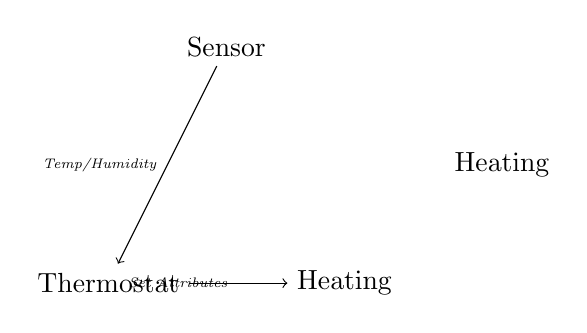
\begin{tikzpicture}
      \node[draw=white,align=left] (S) at (1.5,3) {Sensor};
      \node[draw=white,align=left] (T) at (0,0) {Thermostat};
      \node[draw=white,align=left] (H) at (3,0) {Heating};
      \node[draw=white,align=left] (E) at (5,1.5) {Heating};
      
      \path [->] (S) edge node[left] {\tiny \textit{Temp/Humidity}} (T);
      \path [->] (T) edge node[left] {\tiny \textit{Set Attributes}} (H);
      % \path [->] (H) edge node[left] {} (S);
   \end{tikzpicture}
   
   \caption{Heating System - exercise 2 Schema}
   \label{fig:zigbee_heatingsystem}
\end{figure}
\chapter{Networking}
The two key aspects of a network are:
\begin{enumerate}
   \item \textbf{Bandwidth} $\longrightarrow$ amount of data per second that can be moved through a specific connection
   \item \textbf{Latency} $\longrightarrow$ is the amount of time required for trasmitting data, measured from the moment it is sent from the source to the one it is available to the source.
\end{enumerate}
Latency ---in a datacenter--- to transmit data on the cable using \textit{``pure ethernet''} is of the order of $0.5\times10^{-6}s (\mu s)$.\\
If the TCP/IP stack is used (standard application case), latency is about $70-90\mu s$.

Furthermore, current drives have reached speeds such that latency may act as bottleneck between them and the CPU.

Cable aggregation (e.g. aggregating 4 cables 10Gbit/s, providing 40Gbit/s total)can be performed only at a low ---physical--- level. Otherwise the TCP/IP stream will be associated to a single cable of the ones aggregated, resulting in less bandwidth.

\section{SDN - Software Defined Networking}
SDN is a new approach to networking that uses software-based controllers or application programming interfaces (APIs) to communicate with the underlying hardware infrastructure and direct traffic on the network.

In general a Software Defined Approach aims to abstract all the infrastructure components (compute, storage and network), and pools them into aggregated capacity.

When such approach is applied to a whole datacenter, it is called \textbf{Software Defined Datacenter}, and it is a way to abstract all the infrastructure components in order to provide IT as a service.

\subsection{Hyperconverged Infrastructure (HCI)}
HCI is a software-defined IT infrastructure that virtualizes all of the elements of conventional hardware-defined systems. HCI includes, at a minimum, virtualized computing (a hypervisor), a virtualized SAN (software-defined storage) and virtualized networking (software-defined networking).

\section{Layers}
Programmers usually do not care about anything under layer 3/4 traffic.
However, in datacenters it is fundamental to understand how layer 2 works.
\note{Also because in datacenters there are no routers doing the work for you; you are building the fabric in the first place.}

Layer 2 is fundamental for 2 reasons:
\begin{enumerate}
   \item East-west is Ethernet in the datacenter
   \item All the dozens of protocols used in swithces are really used, so they are important.
   \item MTU - Maximum Transmission Unit
\end{enumerate}

\subsection{Protocols inside switches}
\begin{itemize}
   \item LLDP Link Layer Discovery Protocol - Allows to reconstruct at least partially the functioning of the network.4
   \item DCBX Data Center Bridging Exchange - A meta-protocol so that two devices can agree on the configuration of a bunch of protocols, tipically related to storage/data 
   \note{e.g. ``I need 50\% percent of the bandwidth otherwise a can't work''.\\
   It represents part of some kind of QoS for Ethernet}.
   \item PFC Priority Flow Control
   \item ETS Enhanced Transmission Selection
   \item RSTP Rapid Spanning Tree Protocol - Uses BPDU packets to explore the graph of the network and compute the spanning tree of the network and detect the ---malicious--- cycles if any.
\end{itemize}

This just to recall that \ul{the switch is not a stupid thing}! It is complex, fascinating, and deserves love; it's crucial to understand its functioning, also because its protocols occupy bandwidth.

\section{Ethernet Topology}
Typically nowdays the network is a \textbf{graph}, where internal nodes are switches or routers, and the leaves are servers.

The phyisical medium is no more shared, but conceptually the data link layer behaves as if it was.

On a switch, the only way to emulate a \textbf{shared bus}, is to \textit{``\textbf{copy-paste}''} a frame onto multiple ports, losing the ``identity'' of frames; there is not routing table at layer 2. Packets in higher layers (IP?) have an ID, but frames don't, making it impossible to recognize whether a frame is a copy of another one or not.
This approach makes \textbf{loops} a problem, because they disrupt performance by generating a packet storm.\\
The solution would be to ensure that the topology resembles a \textbf{tree}, instead of a graph.
\ul{But}, at the same time, \ul{a \textbf{fully connected graph}} allows to have \ul{multiple routes for the same destination}, possibly \ul{enhancing performance}, reducing ``hops'' before reaching the destination.

\subsection{\texttt{RSTP}}
\begin{center}
   \textit{So\dots how can we leave the graph to be connected, but making it a tree from a logical point of view?}

   The answer is the \texttt{RSTP} protocol.
\end{center}

RSTP sends \textit{probes} to understand whether there are loops and where are PCs located.
In case of link failure, RSTP is able to adjust the logical tree, blocking the link that caused the loop.

RSTP can be used in campus networks or other networks exhibiting primarily North-South traffic, but it is not suitable for datacenters, where the traffic is mainly East-West:
the protocol is too slow (order of \textit{seconds})to handle the high number of links and the high number of switches typical of a datacenter.

\subsection{Three-tier architecture}
\begin{paracol}{2}
   
   Simple architecture consisting of\ns
   \begin{enumerate}
      \item Core switches
      \item Aggregation switches
      \item Access switches
   \end{enumerate}\ns
   The switches are connected in a tree-like topology, with the core switches at the top, the aggregation switches in the middle, and the access switches at the bottom.\\
   STP is used to prevent loops in the network.

   Also provides active-passive redundancy which leads to inefficient east west traffic, because the traffic is forced to go through the core switches (?), and devices connected to the same port may contend for bandwidth.\\
   Moreover communication server-to-server might requires crossing between layer, causing latency and the abovementioned traffic bottleneck.
   
   \switchcolumn
   
   \colfill
   \begin{figure}[htbp]
      \centering
      \includegraphics{images/3tier_switches.png}
      \caption{Three-tier architecture schema}
      \label{fig:3tier_switches}
   \end{figure}
   \colfill
   
\end{paracol}
This architecture is not used anymore, because it is not scalable, and it is not able to handle the high number of links and switches typical of a datacenter; more specifically, it does not fit virtualization most crucial need to be able to freely move VMs between servers.

\subsection{Spine Leaf architecture}
\begin{figure}[htbp]
   \centering
   \includegraphics{images/spineleaf.png}
   \caption{Spine-leaf architecture schema (from \href{https://www.arubanetworks.com/faq/what-is-spine-leaf-architecture/}{Arubanetworks.com})}
   \label{fig:}
\end{figure}
A \textbf{spine-leaf} architecture is data center network topology that consists of two switching layers:
\begin{enumerate}
   \item \textbf{Spine layer}\\
   Swtiches responsible for routing traffic, working as the backbone of the network.   
   \item \textbf{Leaf layer}\\
   Switches connected to endpoints, such as servers, storage devices, firewalls, load balancers, edge routers, etc.
\end{enumerate}
Since \ul{every leaf switch is connected to every spine switch}, the spine-leaf architecture is a \textbf{fully connected} network,
ensuring that any source is always the same number of hops (actually only one \smiley) away from any destination, so latency is lower and predictable (fixed).

Capacity also improves because STP is no longer required. While STP enables redundant paths between two switches, only one can be active at any time. As a result, paths often become oversubscribed. 
Conversely, spine-leaf architectures rely on protocols such as \textit{Equal-Cost Multipath} (\texttt{ECMP}) routing to load balance traffic across all available paths while still preventing network loops.

Spine-leaf allows \textit{scale-out} opposed to \textit{scale-up}, by adding additional spine switches, ultimately increasing capacity in case the bandwidth is not enough; doing so reduces also the subscription

\subsubsection{LACP}
Loops are prevented using \texttt{LACP} (\textit{Link Aggregation Control Protocol}), which is a protocol that allows to aggregate multiple links into a single logical link, providing higher bandwidth and active-active redundancy (in case a link fails);
it also ensures no loops because each link is a single channel, and these are named \textit{port channels}.

LACP also provides a method to control the bundling of several physical ports together to form a single logical channel.

Note that even though the bandwidth is aggregated (i.e. $2\times 25Gbps$), the single stream is still limited to the bandwidth of a single link (i.e. $25Gbps$), because the traffic goes only from one way to the other each time.

\subsubsection{Advantages of Spine-Leaf}

\begin{itemize}
   \item Modular (because you can mix and match devices) with fixed size switches.
   \item Latency predictable: every host is distance one or two hops to each other host.
   \item Bandwidth control (it's possible to chose the proportion of NS and EW traffic) and overbooking (overbooking explained after).
   \item Active-active redundancy (because both links of the port channels are enabled, so is the LACP to decide)
   \item Loop aware topology (a tree topology with no links disabled for redundancy reasons).
   \item Interconnect using standard cables (decide how many links use to interconnect spines with leaves and how many others link to racks).
   
\end{itemize}
With this architecture it’s possible to turn off one switch, upgrade it and reboot it without compromising the network. Half of the bandwidth is lost in the process, but the twin switch keeps the connection alive.

A typical configuration of the ports and bandwidth of the leaves is:
\begin{itemize}
   \item 1/3 going upwards and 2/3 going downwards
   \item 48 ports 10 Gbps each (downward - from leaves to racks)
   \begin{itemize}
      \item plus 6 ports 40 Gbps each (upward - from leaves to spines)
   \end{itemize}
   \item or (typical switch) 48 ports 25 each (downward)
   \begin{itemize}
      \item plus 6 ports 100 each (upward)
   \end{itemize}
\end{itemize}

Just a small remark: with spine and leaf we introduce \textbf{more hops}, so more latency, than the chassis approach. The solution for this problem is using as
a base of the spine a huge switch (256 ports) which actually acts as a
chassis, in order to reduce the number of hops and latency.


\subsection{Full fat tree}
In a ---full?--- \textbf{fat tree}, branches nearer the top of the hierarchy are "fatter" (thicker) than branches further down the hierarchy. In a telecommunications network, the branches are data links; the varied thickness (bandwidth) of the data links allows for more efficient and technology-specific use.

Full-fat tree is rarely needed.

\section{Virtualization}

With VLAN frames are extended by 4 bytes. Every switch nowdays automatically sets the \texttt{VLAN\_ID} to \texttt{1}; if the field is not existent, it is appended, making an \textbf{tagged} an \textit{untagged} frame.

Switches ensure that data cannot spill/leak from a VLAN to another.
VLAN became largely of use when 10Gbit connection came out, because only 1Gbit was a too constrained bandwidth to be splitted into multiple VLANs. 

VLAN are used to partition the traffic at data link layer without having to redo the fabric. They are particularly useful in cloud environments.

\section{Network Administrator POV}
The switch is split in two planes:
\begin{itemize}
   \item \textbf{Control Plane}\\
   This plane is necessary to configure the data plane to make it behave according to our needs.
   Here there is an \textit{OS}, which used to be proprietary with a functioning fitting a specific network configuration, but nowdays they are usually more configurable and may even be \textit{open} OS.
   \note{\textit{Dell}'s switches now have an \textit{open} OS on board.}
   
   \item \textbf{Data Plane}\\
   Here lies the chip responsible to perform all the data link operations required, runs protocols, handles VLANs, etc.

   \textbf{OpenFlow} allows us to manage the flow table inside of a switch.
\end{itemize}

The two planes are linked by a low-bandwidth PCIe.


It is possible to use a very fast and simple ---reduced number of keystroke down to the strict necessary ones (e.g. \texttt{en} instead of \texttt{enable})--- CLI to program a switch. It is also possible to create a script file to be automatically executed by the switch at boot time.
\note{Prof. Cisternino performed a demo of this in class.}

Interestingly, the behaviour of the \texttt{netsh} command in Windows is very similar to the one of a switch.

\section{SDN}
\textbf{Software Defined Networking} is a new approach to networking that uses software-based controllers or application programming interfaces (APIs) to communicate with the underlying hardware infrastructure and direct traffic on the network.

The problem was that the network infrastructure was ``ossified'' and not programmable. SDN allows to program the network, and to make it more flexible and adaptable to the needs of the applications, without having to disrupt the existing infrastructure.

The key idea proposed in the OpenFlow article, which eventually became a standard, is to separate the control plane from the data plane, and to have a controller that can program through an API the data plane, where the \textbf{Flow Table} resides.

An interesting use of OpenFlow was implemented by a University and called Sandwich firewall, which consisted in routing the first part of the stream through a firewall and if the stream was not malicious, it was routed directly to the destination, otherwise it was dropped.

\subsection*{Latency-sensitive}
Some workloads are called \textit{latency-sensitive}, making the latency introduced by TCP-IP stack a problem.\\
Inside a datacenter nowadays the typical latency is sub microsecond.

Regarding this issue, technologies mentioned earlier come in handy; 
\textit{InfiniBand} is a fabric technology that allows to have a very low latency, and is used in HPC\footnote{High performance computing} environments, and \textit{OmniPath} is a technology that is similar to InfiniBand, but is more scalable and is its natural successor.
Also \textit{RDMA} and \textit{RoCE} are technologies that allow to access memory of a remote machine without involving the CPU or the OS of the remote machine, bypassing the TCP/IP stack.

\textit{Fibre Channel} switches are used in storage area networks, and are used to connect storage to servers CPUs. They are used in datacenters, but not for networking.
\chapter{Blockchain}
The basic concepts concerning Blockchains are
\begin{itemize}
   \item \textit{Ledger}
   \item \textit{Consensus} in a distributed environment
   \item Tamper freeness
   \item Proof of ownership
   \item Permissioned and permissionless blockchains
\end{itemize}

Each \textbf{block} is made up of \textit{Data}, \textit{Hash} and the \textit{Hash of the previous block}; pointers to the previous block are used to ensure the \textbf{order} of the blocks, resulting in a \textbf{chain} of blocks.

\textbf{Tamper freeness} refers to changing one hash causes changing the hash of the following blocks, implying not only to recompute some hashes, but also to find a value that combined with the new hash solves the \textit{Proof of Work}.

\begin{figure}[htbp]
   \centering
   \includegraphics{images/hashpointers.png}
   \caption{Hash pointers and hash of the block prevent attackers from tampering with the blockchain}
   \label{fig:hashpointers}
\end{figure}

A \textbf{ledger}\footnote{\textit{``Libro mastro''} in italiano} acts like a notary, and is replicated on each node of a P2P network, it is immutable and benefits of the tamper freeness property.\\
The ledger is like a bullettin storing operations and their order. It must be an \textbf{append-only} list of events, and also \textbf{tamper-proof}.

\begin{center}
   \ul{If a ledger is organized as a list of blocks, we call it a \textbf{blockchain}}.
\end{center}
\nl

\section{Consesus and challenges}
\textbf{Consensus} is the mechanism which defines who decides which operation will be added to the blockchain, and which operation among those to be confirmed will be added.
Consesus is implemented by \textit{voting}, but there a few things to handle to avoid double spending and fake votes.
\textit{Sybil} attacks are a common issue in voting systems, where a single node can fake multiple identities to gain more voting power.

The two main challenges for the ledger are keeping consistency in case of network jitter and possible delays, and avoid nodes to fake results.
An idea is to establish \textit{consensus} using a \textbf{Proof of Work}, which requires the voting system to be hardly fakeable, i.e. resolving a difficult computational problem.
Enforcing a \textit{PoW} is a way to avoid the Sybil attacks issue, as it implies to have a lot of computational power to fake a vote.\\
The Proof of Work is often compared to a lottery, where tickets for the lottery are very expensive (computational power), and the winner is the one who solves the problem first, and gets the right to decide which block to add to the blockchain.

In case multiple winners are picked at the same time, a \textbf{fork} is created, and the network must decide which fork to follow. The longest fork is usually the one to be followed, as it is the one with the most computational power behind it.

\section{Restricted access}
It is possible to build a permissioned blockchain, where only a restricted set of nodes can vote and add blocks to the blockchain. This is useful in case of a consortium of companies, where the blockchain is used to store transactions between them.

The blockchain may be exploited to demonstrate the validity of the supply chain of a product, or to store the history of a product, from the raw materials to the final product, allowing also to determine which point in the supply chain a product has been compromised.
\chapter{Reflection}
\section*{9 - Ottobre}
\section{Introduction and Definitions}

\textbf{Reflection} is the ability of a program to manipulate as data something representing the state of the program during its own execution.
Another dimension of reflection is if a program is
allowed to \textbf{read only}, or also to \textbf{change} itself.
\begin{itemize}
    \item \textbf{Introspection} is the ability of a program to observe and
    therefore reason about its own state
    \item \textbf{Intercession} is the ability for a program to modify its
    own execution state or alter its own interpretation or
    meaning
    \item \textbf{Reification} is the mechanism of encoding execution state into data, which is needed by both \textit{introspection} and \textit{intercession}
\end{itemize}.

\textbf{Structural} reflection  is concerned with the ability of the \textbf{language} to provide a complete \textit{reification} of both the \textit{program} executed and its \textit{abstract data types}.\\
\textbf{Behavioral} reflection is concerned instead with the reification of its\footnote{referred to a \textbf{language}} \textit{semantics} \& \textit{implementation} (processor) and the data and implementation of the \textit{run-time system}.

\section{Uses and drawbacks}
\subsection{Uses}
\begin{itemize}
    \item \textit{Class Browsers} need to be able to enumerate the number of classes
    \item \textit{Visual Development Environments} can exploit type info available in reflection to aid the developer in writing correct code
    \item \textit{Debuggers} need to be able to examine private members on classes
    \item \textit{Test Tools} exploit reflection to ensure a high level of code coverage in a test suite
    \item \textit{Extensibility Features} an app may make use of external, user-defined classes by creating instances of extensibility objects.
\end{itemize}

\subsection{Drawbacks}
\begin{itemize}
    \item \textbf{Performance Overhead}
    \item \textbf{Security Restrictions}
    \item \textbf{Exposure of internals}
\end{itemize}

\section{Reflection in Java}
Java supports \textbf{introspection} and \textbf{reflexive invocation},
but not \textit{code modification}.

\subsection{Introspection}

The JVM mantains for every type an associated object of type \lstinline{java.lang.Class} which "\textit{reflects}" the type it represents,
acting as entry point for reflection,
since it provides all info needed:
\begin{itemize}
    \item Class name and modifiers
    \item Extended superclasses and implemented inferfaces
    \item Methods, fields, constructors, etc.
\end{itemize}

To retrieve such \lstinline{java.lang.Class} object it is sufficient to do \lstinline{Object.getClass()}.
\lstinline{Class} objects are constructed automatically by the JVM as classes are loaded.

Using \lstinline{java.util.reflect.*} it is possible also to retrieve class \textbf{Members} i.e. \textit{fields, constructors} and \textit{methods}.
The extensive \lstinline{java.util.reflect.*} API provides many \textit{methods} to achieve this which will not be reported here.\\
There is a class for each Member
\begin{itemize}
    \item \lstinline{java.util.reflect.Field}: access type info and set/get values.
    \item \lstinline{java.util.reflect.Method}: type info for parameters and return type;
    invoking method on a given object.
    \item \lstinline{java.util.reflect.Constructor}: note that constructors have no return values and invocation creates a new instance of the given class.
\end{itemize}

\subsection{Program Manipulation}
By now we have talked only about \textbf{introspection} in java,
but reflection can be used also to create objects of a type not known at compile time,
or to access members (access fields or invoke methods) unknown at compile time.


\chapter{Virtualization}

Virtualization consists in virtualizing hardware resources, such as CPU, memory, storage, and network interfaces. This allows to run multiple operating systems on the same physical machine, which is called \textit{host}.

It is not equal to \textit{emulation} which consists in simulating hardware, giving the illusion that you are in another system, and is much slower than virtualization, since each instruction in the emulated system gets translated into up to ---possibly--- thousands  of instructions in the host.

\framedt{CPU Rings and isolation}{
   \ul{Virtualization is a strong way of isolating things.}\\
   To isolate VMs the hypervisor exploits CPU rings, which are used to separate the different levels of privilege. The higher the ring, the higher the privilege level.
   In intel CPUs there are 16 rings.
}

There are two kinds of virtualization systems:
\begin{enumerate}
   \item VirtualPC (Microsoft), VirtualBox (Oracle), VMware Workstation (VMware), Parallels (Apple) : these are \textit{desktop virtualization systems}, which are used to run multiple operating systems on the same physical machine.\\
   These solutions aim to provide ``interactive'' computers, with a GUI, peripheral support, etc. 
   \item VMware ESXi, Microsoft Hyper-V, KVM, Xen : these are \textit{server virtualization systems} (\textbf{HyperVisors}), which are used to run multiple servers, typically GUI-less, on the same physical machine.\\
   Hypervisors introduce a \textbf{crucial} piece of software called \textbf{Virtual Switch}, which is responsible for managing the network of the virtual machines.
   The virtual switch's uplink is the host's physical network interface.
\end{enumerate}
Similarly to snapshots in storage systems, there are \textbf{checkpoints}, which are used to save the state of a virtual machine at a certain point in time. This is useful to revert to a previous state in case of problems.

\section{Network}
HyperVisors introduce a \textbf{crucial} piece of software called \textbf{Virtual Switch}, which is responsible for managing the network of the virtual machines.\\
VMware is the leader in virtualization, but lately they have been changing pricings and licensing, which has made some customers unhappy.\\
\note{Broadcom is a chip manufacturer, and we might end up with virtualization software already inside the chip. }

VMware virtual switch is called \textbf{vSwitch}. It is a software-based switch that is responsible for managing the network of the virtual machines.\\
Every network interface of a virtual machine has its own MAC address, and may be connected to a vSwitch.
\note{An hypervisor may handle multiple vSwitches.}
From a network point of view, a virtual machine is just like a physical machine, assuming that the network card is in \textbf{promiscuous} mode, it can see all the traffic that is going through the vSwitch.

\section{Live Migration}
Hypervisors provide also the migration of virtual machines from one host to another, which is called \textbf{vMotion} in VMware. This is useful for load balancing, maintenance, etc. In Windows Hyper-V, this primitive is called \textbf{Live Migration}.\\
The migration is performed \textit{without any service interruption}, only some degradation in performance and network latency.
This also allows to move virtual machines from one host to another in case of hardware failure or phyisical maintenance.
Besides, by redunding VMs we may also live switch from an older to a newer version of the software, without users noticing.

Live migration can performed like a context switch, by saving the state of the virtual machine and restoring it on the other host. This is possible because the virtual machine is not aware of the underlying hardware, and the hypervisor is responsible for managing the hardware resources.\\
Assuming that the disk is shared, the migration is performed like so:
\begin{enumerate}
   \item The memory (and the registries) of the virtual machine is copied to the other host
   \item If the copied memory is sufficient, the new VM starts to run on the other host
   \item When data from the older memory host is requested, the virtual machine is paused, and the memory is copied again to the other host
   \item Once the VM has been totally transferred, memory and other components belonging to the old VM are freed
\end{enumerate}

vSwitches are also migrated, so that the network configuration is preserved. The old vSwitch may communicate with the new one, and if needed forward packets, until ARP tables are updated.

\subsection{Replication}
Replication is the process of copying data from one host to another, in order to have a backup in case of failure.\\
Happens the same way as live migration, but the virtual machine is not running on the other host.
\chapter{Bitcoin Mining}

Recall that the \textbf{distributed consesus} is a procedure to reach a common agreement in a distributed or decentralized multi-agent system;
it must ensure correct results even in presence of faulty nodes, network partitioning and byzantine faults\footnote{Nodes behaving maliciously}.
\note{Even though it is difficult to classify the method used by Bitcoin to achieve decentralization from a theoretical point of view, it works in practice.

\textit{``...is not purely technical, but it's a combination of technical methods and clever incentive engineering.''}
}

\section{Competing}
Every node holds a \texttt{MemPool} containing all Bitcoin transactions awaiting confirmation.
\ul{\textit{Conflicts} may happen there, not in the ledger}.
In case a node receives a double-spending transaction, it will keep the first one and discard the second one.\\
Nodes try to get transactions into the ledger, and \textbf{compete} to do so.
Nakamoto consesus is implemented like a ``lottery'' where the winner gets to add a block ---of valid transactions--- to the blockchain, and to send its neighbours the updated ledger. The process of competing to add transactions to the blockchain is called \textbf{mining}.

\subsection{Mining}
Mining process starts with filling a candidate block with transactions taken
from the memory pool (\texttt{MemPool}), and then building a block header (1000 times smaller than the block);
finally the node performs the Proof of Work.\\
So, while a single transaction may be built by anyone, blocks are built by miners, and include multiple transactions and the header.

\begin{paracol}{2}
   \ns
   The block header contains:
   \begin{itemize}
      \item Version
      \item Timestamp
      \item \texttt{mhash} The Merkle \ul{root} of the transactions in the block
      \note{Merkle tree is not explicitly represented in the block, it is built on demand.\\
      Any change to a transaction results in a change of \texttt{mhash}, consequently in a change of the hash of the whole block.}
      \item \texttt{hashprev} The hash of the previous block \textit{header}, and a hash pointer to the previous block
      \item PoW related fields:
      \begin{itemize}
         \item Target
         \item Nonce
      \end{itemize}
   \end{itemize}
   \switchcolumn

   \colfill
   \begin{figure}[htbp]
      \centering
      \includegraphics{images/bitcoin_blockheader.png}
      % \caption{}
      \label{fig:bitcoin_blockheader}
   \end{figure}
   \colfill

\end{paracol}

\framedt{Mining}{
   \begin{enumerate}
      \item Set \texttt{nonce = 0}
      \item Hash the \textit{block header} including the \texttt{nonce}
      \item \texttt{while (\texttt{hash} > \texttt{target})}
      \begin{enumerate}
         \item Increment \texttt{nonce}
         \item Hash the \textit{block header} including the \texttt{nonce}
      \end{enumerate}
   \end{enumerate}
   \textbf{Target} acts as \textit{threshold}, and represents the \ul{number of leading zeros the hash must have}.
   The nonce is 32 bit long, and even a slight increment on it changes the whole hash result.
}

\subsection{Consesus}
Node is selected to propose the next block in proportion to a resource that it is hard to
monopolize: in Bitcoin this resource is \textbf{computational power} and the selection is done on the basis of the Proof of Work.

The Consensus is \textbf{implicit}:
\begin{itemize}
   \item No collective distributed algorithm executed by the nodes
   \item No voting
   \item Selection of malicious nodes is also implicitily handled by the system
\end{itemize}

Even if the nodes may have occasionally an inconsistent view of the ledger (blockchain forks) consensus will eventually occur, the consistent ledger will eventually be the longest chain.
\note{This is true if the majority of the nodes are honest.}

\subsection{Proof of Work}
\begin{itemize}
   \item \texttt{d} - \textit{difficulty}: a positive number which is used to adjust the time to execute the proof
   \item \texttt{c} - \textit{challange}: a given string (the block header minus the nonce)
   \item \texttt{x} - \textit{nonce}: an unknown string
\end{itemize}

\begin{definition}[Proof of Work]
   A proof of work is a function $F_d(c,x) \rightarrow {\texttt{True,False}}$ satisfying:
   \begin{enumerate}
      \item \texttt{d} and \texttt{c} are \textit{fixed}
      \item $F_d(c,x)$ is \textit{fast to compute}, if \texttt{d}, \texttt{c}, and \texttt{x} are known
      \item instead, finding \texttt{x} so that $F_d(c,x) = \texttt{True}$ is computationally difficult, but feasible.
   \end{enumerate}
\end{definition}

The PoW is hard to solve because the computing output looks like a random 256-bit string where each bit is equally likely to be \texttt{0} or \texttt{1} independently of the other bits, so each output bit looks like coin flips (\texttt{0/1}).
There is no better way of finding the correct output than trying by \textbf{brute force}.\\
The probability $p$ that the block hash is below the target $T$ and average number of attempts $a$ to find a solution are:
\begin{align*}
   p=\frac{T+1}{2^{256}} & & a=\frac{1}{p}
\end{align*}

The system is resistant to Sybil attacks because the PoW is a scarce resource, and the cost of the attack is proportional to the whole computational power of the attacker, not to the number of identities they have.

\note{The Proof of Work is also used in other contexts to prevent spam, like in Hashcash, and to counter DoS attacks, by allowing users to access a service only after solving a PoW.

Email spam may be prevented through a PoW by adding a post stamp to each email message, and the receiver may decide to accept the message only if the PoW is valid.}

\subsection{Block propagation and incentives}
\subsubsection{Block propagation}
The mined block is broadcasted on the network, and each node receiving the block verifies that the PoW has been solved by hashing the block header and checking that the hash is less than the target.
It is easy to verify, without centralization points.\\
After the verification, the node adds the block to the blockchain and kicks out any conflicting transaction from \texttt{MemPool}.

\subsubsection{Incentives}
There are two mechanisms to incentivize the miners to be honest:
\begin{enumerate}
   \item \textbf{\ul{Block reward}}:
   a payment to the miner in exchange for the service of creating a block.\\
   Bitcoin mints new coins when a new block is mined, and is the only way to create new bitcoins.\\
   The reward is halved every 210K blocks ($\sim 4 \textit{ years}$), and the last block reward will be mined in 2140.
   \item \textbf{\ul{Transaction fees}}:
   for each transaction in the block the miner gets the difference between transaction inputs and outputs.\\
   It was voluntarily inserted to obtain a good ``quality of service'' from the miners.
\end{enumerate}

The first transaction in each block is called \ul{\textbf{coinbase transaction}, and is the one that mints new coins}: it includes the reward plus the transaction fees to the miner, and is not linked to any previous UTXO, but to a single ``dummy'' input.

\framedt{Mining Difficulty}{
   \begin{center}
      \textit{``To compensate for increasing hardware speed and varying interest in running nodes over time, the proof-of-work difficulty is determined by a moving average targeting an average number of blocks per hour. If they're generated too fast, the difficulty increases.''}\\
      -Satoshi Nakamoto
   \end{center}
   The difficulty is adjusted every 2016 blocks (about 2 weeks) to keep the block time around \textbf{10 minutes}.
   The difficulty is adjusted by changing the target, which is inversely proportional to the difficulty.
}

\framedt{Why 10 Minutes?}{
   \begin{center}
      \textit{``If broadcasts turn out to be slower in practice than expected, the target time between blocks may have to be increased to avoid wasting resources. 
      We want blocks to usually propagate in much less time than it takes to generate them, otherwise nodes would spend too much time working on obsolete blocks.''}\\
      -Satoshi Nakamoto
   \end{center}

   The 10 minutes target time is a trade-off between the time to propagate a block and the time to generate a new one.\\
   The goal was to allow time to propagate across the whole network before the next block gets mined, to avoid wasting resources.
}

Note that 10 minutes mining time means that no instantaneous transactions are possible, but the system is designed to be secure, not fast.
\note{e.g. you can't pay for an ice cream using bitcoin.}

\begin{figure}[htbp]
   \centering
   \includegraphics{images/bitcoin_targetcycle.png}
   \caption{Bitcoin target cycle}
   \label{fig:bitcoin_targetcycle}
   \note{A node can't avoid decreasing the target, since the other nodes would not validate its Proof of Work.}
\end{figure}

\note{Blocks are preferred over single transactions, because verification is faster and mining single transactions would overall require more mining work.}

\subsection{Tamper-freeness}
The blockchain is tamper-free because:
\begin{itemize}
   \item The PoW is hard to solve
   \item The PoW is easy to verify
   \item The PoW is a scarce resource
\end{itemize}

\newpage
It would take an \ul{unfeasible amount of power for an attacker to change a transaction in a block}, since it would imply that: 
\begin{enumerate}
   \item The root of the Merkle tree changes and so the block header
   \item The nonce of the block is no more valid
   \item Re-execute PoW to re-compute the right nonce for the new block
   \item In the next block the hash pointer to the previous block changes as well
   \item Nonce of the next block is no more valid
   \item Need to re-execute also on next block...
   \item ...and so on
\end{enumerate}

\section{Temporary Forks}

\begin{paracol}{2}
   
   \colfill
   \ul{Temporary forks may happen when two miners find a valid block at the same time}, and broadcast it to the network.
   The state of the blockchain is seen by the nework consists of two branches both
   originating from the same parent block.
   In this case both branches are legitimate, and is different from the double spending case, but still, \textit{which bitcoin are really spent?}
   \colfill

   \switchcolumn

   \colfill
   \begin{figure}[htbp]
      \centering
      \includegraphics{images/bitcoin_forks.png}
      \caption{Bitcoin temporary forks}
      \label{fig:bitcoin_forks}
   \end{figure}
   \colfill
\end{paracol}
   

Each miner node either receives block A or block C first, which are both valid, but different,
and then starts mining on the branch of the fork with the block it received first;
note that the two forks may grow indipendently, and the network may have multiple branches.
If a \ul{miner receives a block that makes the other fork longer, it \textit{abandons} the
shorter fork};
the transactions of the ``abandoned'' fork that were not approved in the winning fork are returned to the pool of ``not-yet-approved'' transactions.
\begin{definition}[6 Confirmation Rule]
   \label{def:6confirmation}
   Bitcoin approves a transaction finally only once there are at least \textbf{five} following blocks in the chain 
\end{definition}

\framedt{May the two chains extended perfectly in parallel, to equal height?}{
   It may be possible, but extremely unlikely in practice.
   The probability that this happens recursively, for a long period is very low,
   besides mining and the block propagation delay introduce randomness in the protocol that typically prevents this.

   Recall that each miner switches to mine on the longest branch it becomes aware of.
}

\begin{definition}[Nakamoto Consesus]
   Forks are \textit{eventually} resolved and all nodes eventually agree on which is the longest
   blockchain. The system therefore guarantees \textbf{eventual consistency}.
\end{definition}

\section{Mining technologies}
The main Bitcoin actors are:
\begin{enumerate}
   \item Reference client (Bitcoin Core)
   \item Full block chain mode
   \item Solo miner
   \item Lightweight (SPV) wallet
\end{enumerate}

Basically, the mining process is SHA computation which can be summarized as follows:
\begin{lstlisting}
   while (1)
      HDR[kNoncePos]++;
      if (SHA256(SHA256(HDR)) < (65535 << 208)/ DIFFICULTY)
         return;
\end{lstlisting}
To compute such hash, CPUs were initially used, then GPUs,GPU pools, FPGAs ---Verilog programmable hardware--- and now ASICs are used.
It is unclear what will ASICs successor be.
ASICs stands for Application Specific Integrated Circuits, and are hardware devices specifically designed to perform a task, e.g. mining.
For this task, they are faster and more efficient than CPUs and GPUs.

\subsection{Centralized Mining pools}
\label{sec:mining_pools}
\ul{Mining is a very risky task}, since it is very likely to spend a lot for mining hardware and eletricity without
obtaining a reward for a long time.
\textbf{Mining pools} are a way to share the risk and the reward among the participants. 

The \textbf{Pool Manager} sends blocks to miners and distributes the reward among the participants, based on the work they have performed; it must be trusted by anyone.
\labelitemize{\textit{Challenges}}{
\begin{itemize}
   \item How does a pool manager know how much work each member of the pool is actually performing?
   \note{Also miners that have not been able to solve the PoW have to be rewarded for their work.}
   \item How can the pool manager divide the revenue proportional to the amount of work each miner is doing?
   \note{Partecipants to the pool may cheat, i.e. claim that they've done more than they actually did.\\
   It is in general hard to prove how much work a node has performed. Generally some ``near-valid blocks'' are sent to the pool manager, to indicate that the miner is actually working.}
\end{itemize}   
}

\textit{Pay-per-share} (PPS) is a common reward system used by mining pools, where the pool manager pays a fixed amount for each share submitted by the miner.
Miner's are payed from pool's existing balance, and there is no special reward for the miner who actually mines the block.

\textit{Pay-proportional} is instead a reward system where the pool manager enacts a reward proportional to the amount of work done by the miner, making miners more incentivized to present valid blocks.
This is less riskful for the pool manager, since payment is enacted only when a block is mined.
\note{\ul{Understading the amount of work done by a miner is still a challenge}. \textit{Decentralized mining pools} are a solution to this problem.}

\newpage
\subsection{Decentralized Mining pools}
\begin{paracol}{2}
   
   The basic idea behind decentralized mining pools is to build a separate, private chain including \textit{``weak blocks''} mined with lower difficulty, store in the private chain called \textit{``sharechain''} transactions rewarding for mining weak blocks
   until a valid block is found;
   at that point reward is distributed through a side blockchain which is then merged to the main chain, hence obtaining a transparent and fair payout scheme with efficiency minimal performance overhead.

   This approach also solves the problem of having a centralization point, since the pool manager does not have to be distribute the rewards.

   \switchcolumn
   \colfill
   \begin{figure}[htbp]
      \centering
      \includegraphics{images/bitcoin_decentralized_pool.png}
      \caption{Sharechain and main bitcoin chain}
      \label{fig:bitcoin_decentralized_pool}
   \end{figure}
   \colfill

\end{paracol}

\end{document}
